\clearpage
\phantomsection

\setcounter{chapter}{2}
\chapter[CÀI ĐẶT VÀ THỰC NGHIỆM]{CÀI ĐẶT VÀ THỰC NGHIỆM}
Chương này mô tả cách hiện thực hệ thống đã thiết kế ở Chương~2, tập trung vào những quyết định kỹ thuật ảnh hưởng đến kết quả thực nghiệm. Trọng tâm là ma trận thí nghiệm loại trừ gồm 9 lần chạy để cô lập tác động từng kỹ thuật, và hai lần chạy mở rộng run59/run62 để kiểm tra nút thắt quan sát. Cấu trúc chương đi từ quy trình PCGNN, hiện thực CombatAgent, cấu hình huấn luyện PPO đến thiết kế thí nghiệm loại trừ.
% \textbf{Bản đồ thực nghiệm.} Trước khi đi vào chi tiết cài đặt, Bảng~\ref{tab:experiment_roadmap} tóm tắt 11 lần chạy sẽ được phân tích ở Chương~4, dán nhãn rõ \emph{thay đổi gì so với cấu hình cơ sở} và \emph{trả lời câu hỏi nghiên cứu/mục tiêu nào}.
\begin{table}[H]
    \centering
    \small
    \caption{Tổng quan các cấu hình thí nghiệm và vai trò phân tích}
    \label{tab:experiment_roadmap}
    \begin{tabular}{|p{1.4cm}|p{4.8cm}|p{4.5cm}|p{3.0cm}|}
        \hline
        \textbf{Run} & \textbf{Thay đổi so với cấu hình cơ sở (run34)} & \textbf{Vai trò phân tích} & \textbf{Mục tiêu} \\
        \hline
        run34 & -- (PPO cơ sở, 207D, không curriculum) & Mốc so sánh & MT1 \\
        \hline
        run35 & + ICM & Đánh giá ICM trong khám phá & MT3 \\
        \hline
        run36 & + RND & Đánh giá RND trong khám phá & MT3 \\
        \hline
        run42 & + LSTM & Đánh giá vai trò bộ nhớ & MT3 \\
        \hline
        run46 & + Curriculum (3 bài học) & Đánh giá curriculum learning & MT2 \\
        \hline
        run47 & + Curriculum + LSTM & Đánh giá bổ trợ của LSTM & MT3 \\
        \hline
        run50 & + Curriculum + ICM & Đánh giá bổ trợ của ICM & MT3 \\
        \hline
        run54 & + Curriculum 4 bậc (Hard Random) & Ảnh hưởng của vị trí sinh & MT2 \\
        \hline
        run55 & + Curriculum + hàm thưởng v2 & Đánh giá thang thưởng mới & MT1 \\
        \hline
        run59 & + Quan sát 210D (path-informed BFS) & Kiểm tra nút thắt biểu diễn & MT4 \\
        \hline
        run62 & + Quan sát 432D (lưới cục bộ 15×15), 40.82M bước & Đánh giá quan sát lưới cục bộ & MT4 \\
        \hline
    \end{tabular}
\end{table}

\section{Môi trường phát triển}

Môi trường game được xây dựng bằng Unity 6 và TopDown Engine. Phần học tăng cường dùng Unity ML-Agents để kết nối cảnh chơi Unity với trainer Python. Các thí nghiệm chính được chạy bằng bản build standalone ở chế độ không đồ họa, với nhiều môi trường song song để tăng tốc độ thu thập mẫu.

\begin{table}[H]
    \centering
    \small
    \caption{Môi trường triển khai và huấn luyện}
    \label{tab:development_environment}
    \begin{tabular}{|p{5cm}|p{8cm}|}
        \hline
        \textbf{Thành phần} & \textbf{Cấu hình sử dụng} \\
        \hline
        Game engine & Unity Editor 6000.1.3f1. \\
        \hline
        Gameplay framework & TopDown Engine v4.4, môi trường demo Koala2D được mở rộng cho bài toán RL. \\
        \hline
        Unity package & com.unity.ml-agents phiên bản 4.0.3. \\
        \hline
        Trainer & Unity ML-Agents Python trainer, thuật toán PPO, log qua TensorBoard. \\
        \hline
        Phần cứng & CPU 16 luồng, RAM 16GB, NVIDIA GeForce RTX 3050 6GB. \\
        \hline
        Chế độ chạy & Build standalone, --no-graphics, time-scale=20, thường dùng 8 môi trường song song; một số run dùng 16 môi trường. \\
        \hline
    \end{tabular}
\end{table}

Việc dùng build standalone thay vì chạy trực tiếp trong Editor giúp giảm nhiễu do giao diện và ổn định tốc độ mô phỏng. Với cấu hình 3 triệu bước, thời gian huấn luyện một lần chạy đầy đủ thường nằm ở khung 4 giờ, trong đó phần tốn thời gian nhất là mô phỏng Unity và đồng bộ nhiều môi trường, không phải forward pass của mạng MLP.

\section{Hiện thực quy trình sinh bản đồ bằng PCGNN}

Quy trình bản đồ được tách thành hai giai đoạn. Giai đoạn ngoại tuyến chạy trong môi trường Python của PCGNN để sinh, đánh giá và chia bản đồ theo độ khó. Giai đoạn trong Unity chạy thông qua TilemapGenerator để nạp bản đồ đã chọn vào lượt chơi huấn luyện. Cách tách này là cải tiến quan trọng so với phương án gọi bộ sinh trực tiếp từ Unity: quá trình huấn luyện ổn định hơn, bản đồ có thể được kiểm tra trước, và người thiết kế vẫn có quyền chọn những bản đồ phù hợp nhất trước khi đưa vào tập huấn luyện chính.

Ở giai đoạn PCGNN, đề tài sử dụng genome đã huấn luyện \emph{winnerseed0.pkl}để sinh bản đồ. Mỗi ô bản đồ được sinh theo thứ tự quét từ trái sang phải, từ trên xuống dưới; mạng nhận ngữ cảnh cục bộ $3 \times 3$ xung quanh ô hiện tại cùng bốn đầu vào ngẫu nhiên, sau đó quyết định ô đó là tường hay sàn. Kết quả sau đó được bộ chuyển đổi chuyển sang text map của game.

Để người đọc có trực giác về sự khác nhau giữa thiết lập PCGNN tham chiếu và biến thể dùng trong khóa luận, Hình~\ref{fig:pcgnn_baseline_vs_improved} đặt cạnh nhau các mẫu bản đồ sinh từ hai genome đại diện. Phía tham chiếu dùng checkpoint \emph{neat\_winner\_seed0.pkl} của notebook \emph{BaseLine.ipynb}, tương ứng với kiến trúc NEAT feed-forward trong nghiên cứu PCGNN. Phía cải tiến dùng checkpoint \emph{winnerseed0.pkl}, tương ứng với bộ sinh recurrent được dùng để tạo tập bản đồ chính cho Unity. Hai bên cùng giữ quy ước P/E, nhưng bản cải tiến tạo ra nhiều hành lang dài và cấu trúc định hướng hơn, phù hợp với mục tiêu tuyển chọn bản đồ cho curriculum.

\begin{figure}[H]
    \centering
    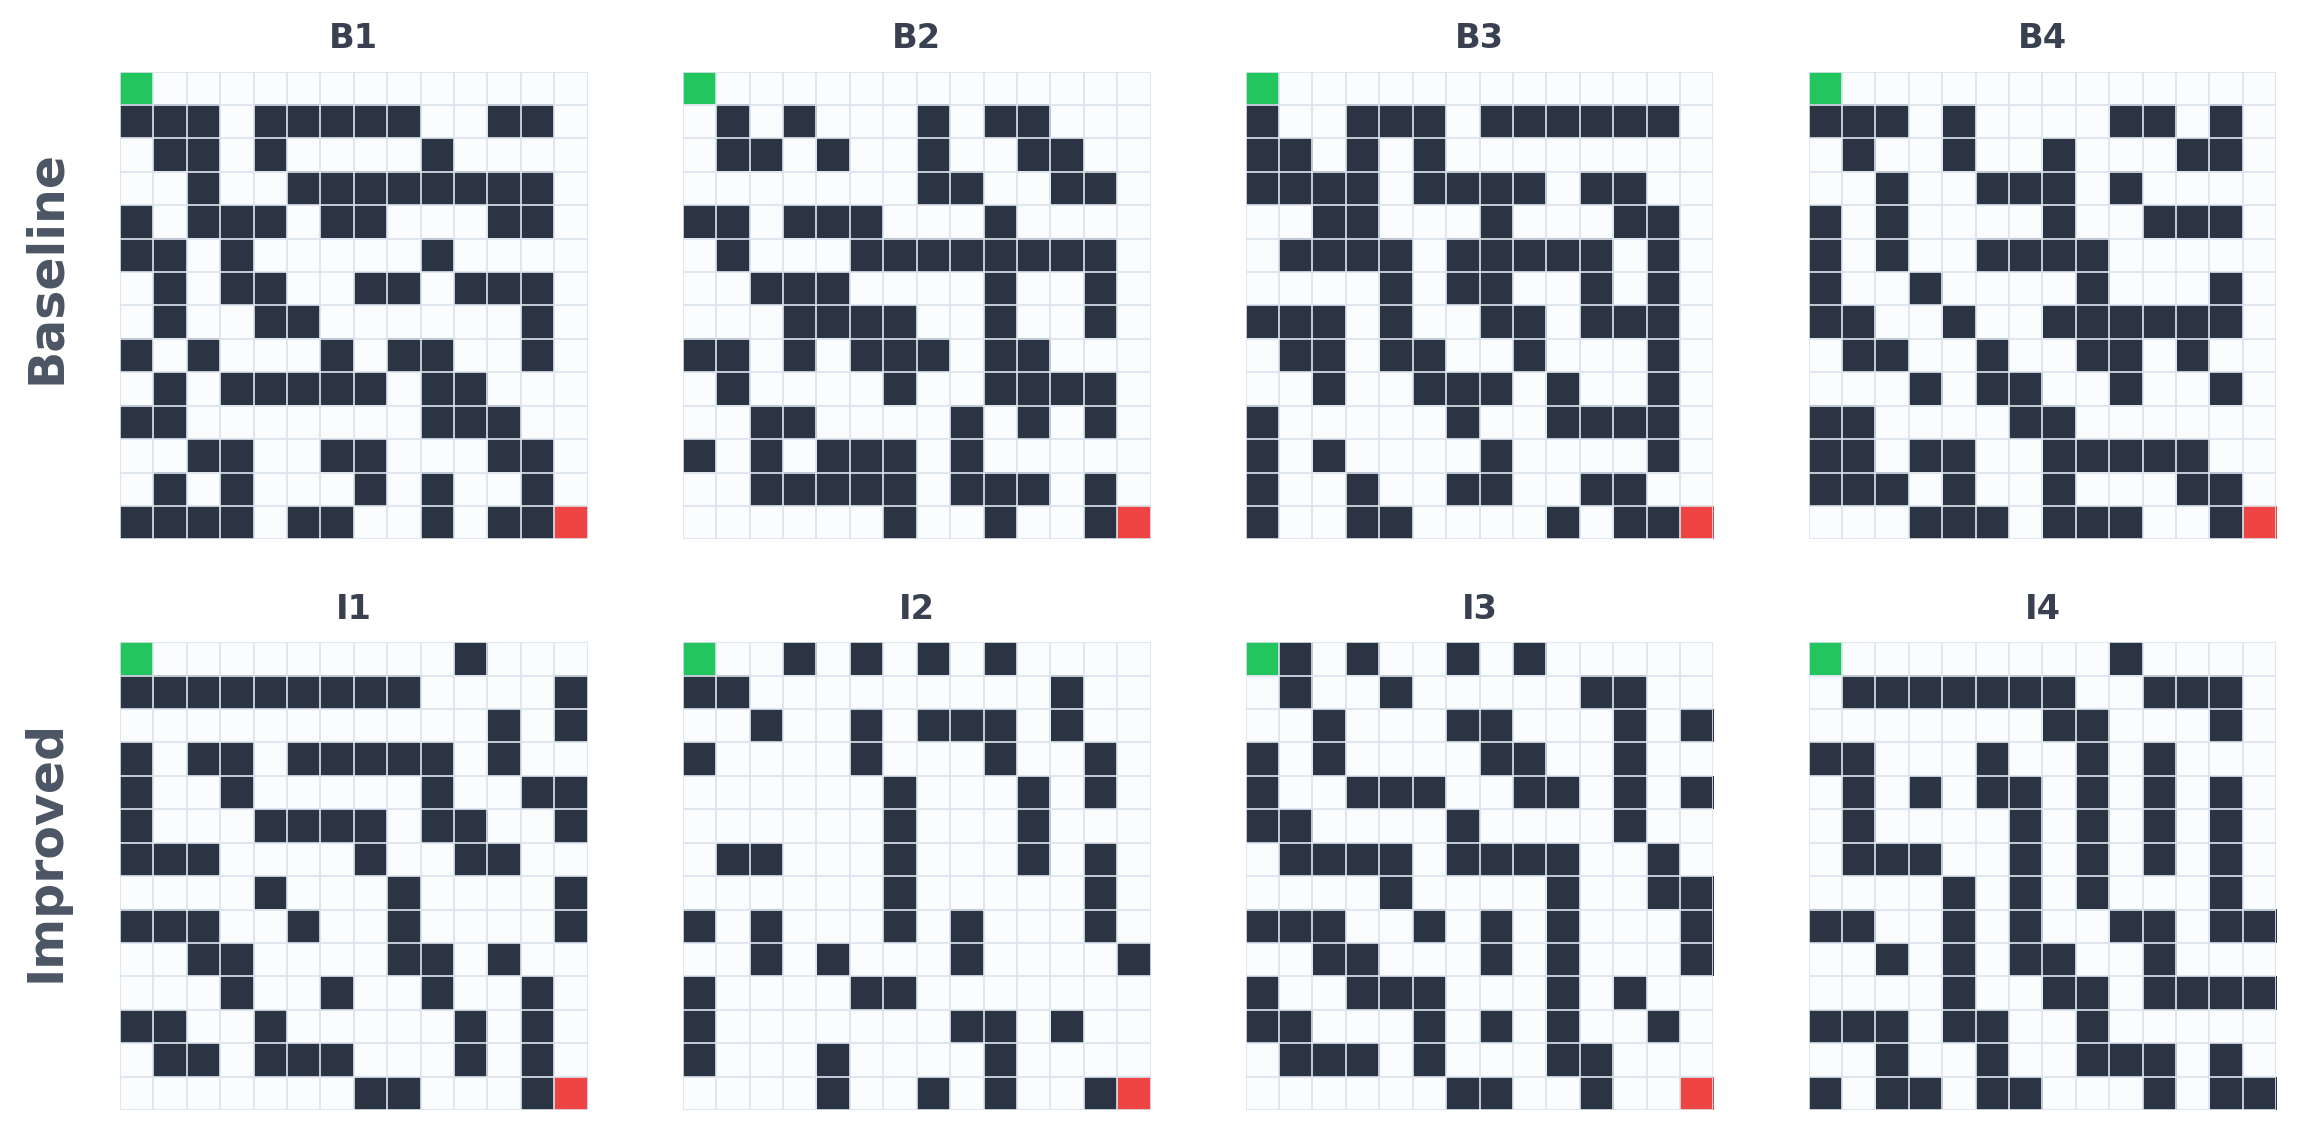
\includegraphics[width=\textwidth]{figures/pcgnn/map_baseline_vs_improved.png}
    \caption{So sánh mẫu bản đồ PCGNN tham chiếu và mẫu bản đồ cải tiến dùng trong khóa luận}
    \label{fig:pcgnn_baseline_vs_improved}
\end{figure}

Hình~\ref{fig:pcgnn_baseline_vs_improved} đóng vai trò so sánh tổng quan giữa hai hướng sinh bản đồ. Các hình ở phần sau sẽ làm rõ hơn hai ý cụ thể: PCGNN tham chiếu thường tạo các đường đi kiểu mê cung nối hai góc, còn bản cải tiến của khóa luận sau bước bộ chuyển đổi sẽ được đánh giá thêm bằng BFS, khả năng đi tới và điểm độ khó trước khi đưa vào các nhóm Easy, Medium và Hard.

\subsection{Điều chỉnh PCGNN cho bài toán Roguelike}

Trong nghiên cứu gốc, PCGNN là bộ sinh level độc lập, được đánh giá bằng leniency, A* difficulty, compression distance và A* diversity~\cite{Beukman2022}. Ở đây, PCGNN được dùng để sinh bản đồ nền cho Unity; các điều chỉnh chính được tóm tắt trong Bảng~\ref{tab:pcgnn_improvements}.
\begin{table}[H]
    \centering
    \small
    \caption{Các điều chỉnh PCGNN trong khóa luận}
    \label{tab:pcgnn_improvements}
    \begin{tabular}{p{4.0cm} p{5.0cm} p{5.0cm}}
        \toprule
        \textbf{Thành phần} & \textbf{Thiết lập PCGNN tham chiếu} & \textbf{Điều chỉnh trong khóa luận} \\
        \midrule
        Vai trò của bộ sinh & Sinh level/bản đồ để đánh giá chất lượng và độ đa dạng của nội dung. & Sinh tập bản đồ ngoại tuyến để đưa vào curriculum learning trong Unity. \\
        Biểu diễn đầu ra & Ma trận tile của miền Maze/Mario trong thiết lập tham chiếu. & Chuyển sang text map của game với ký hiệu \#, ., P, E. \\
        Xử lý vị trí người chơi và kẻ địch & Phụ thuộc vào biểu diễn của từng miền sinh bản đồ. & Adapter đặt P/E trên cùng thành phần liên thông lớn nhất và chọn hai vị trí cách xa nhau. \\
        Kiểm tra hợp lệ & Đánh giá bằng các chỉ số ngoại tuyến. & BFS xác nhận đường đi từ P tới E; TilemapGenerator kiểm tra lại vùng đi được khi nạp bản đồ. \\
        Chỉ số bổ sung & Các chỉ số PCGNN gồm leniency, A* difficulty, compression distance và A* diversity. & Bổ sung các chỉ số reachable\_ratio, dead\_end\_ratio và difficulty\_score để phục vụ chọn bản đồ cho curriculum. \\
        Tổ chức dữ liệu & Không gắn với bài học của môi trường Unity. & Chia bản đồ thành Easy/Medium/Hard theo percentile để điều khiển độ khó huấn luyện. \\
        Tích hợp lúc chạy & Không hướng tới gọi trực tiếp trong Unity. & Tách bộ sinh ngoại tuyến và TilemapGenerator trong Unity để giảm độ trễ, tăng khả năng tái lập và cho phép kiểm tra bản đồ trước. \\
        \bottomrule
    \end{tabular}
\end{table}

Do đó, đóng góp của khóa luận đối với PCGNN không nằm ở việc thiết kế lại thuật toán NEAT, mà ở lớp hậu xử lý, kiểm định khả năng đi tới và tích hợp bản đồ vào curriculum. Hướng tiếp cận này phù hợp với mục tiêu đề tài: tạo tập bản đồ sinh theo thủ tục đủ đa dạng nhưng vẫn kiểm soát được tính hợp lệ trước khi dùng huấn luyện CombatAgent.

\subsection{Adapter và kiểm tra hợp lệ}

Adapter thực hiện ba việc: chuyển ma trận tile của PCGNN sang ký tự \# và dấu chấm (.); tìm thành phần liên thông lớn nhất của vùng sàn và đặt P/E ở hai ô cách xa nhau trong thành phần đó; chạy lại BFS để xác nhận đường đi từ P tới E tồn tại. Nhờ vậy, các bản đồ đưa vào Unity tránh được các lỗi phổ biến của PCG như người chơi bị nhốt, kẻ địch nằm ở vùng không thể tiếp cận, hay bản đồ thiếu ô sàn hợp lệ.

Mỗi bản đồ hợp lệ được ghi ra file .txt, đồng thời một dòng chỉ số được lưu trong file \emph{metrics.csv}. Các chỉ số chính gồm:

\begin{itemize}
    \item \emph{wall\_ratio}: tỷ lệ ô tường trên toàn bản đồ.
    \item \emph{shortest\_path\_length}: độ dài đường đi ngắn nhất từ P tới E.
    \item \emph{dead\_end\_ratio}: tỷ lệ ô đi được có số hàng xóm mở nhỏ hơn hoặc bằng một.
    \item \emph{reachable\_ratio}: tỷ lệ vùng sàn thuộc thành phần liên thông lớn nhất.
    \item \emph{astar\_difficulty}: mức độ A* phải mở rộng thêm node ngoài đường đi tối ưu.
    \item \emph{difficulty\_score}: điểm tổng hợp dùng để sắp xếp bản đồ theo độ khó.
\end{itemize}

Các đại lượng trên được dùng để đánh giá \emph{chất lượng hình học của ma trận bản đồ}, không phải hiệu năng cuối cùng của tác nhân. \emph{wall\_ratio} kiểm soát mật độ vật cản; nếu quá thấp thì phòng gần như trống, nếu quá cao thì dễ tạo vùng bị chia cắt. \emph{shortest\_path\_length} đo khoảng cách di chuyển tối thiểu giữa người chơi và kẻ địch, nên liên quan trực tiếp đến thời gian tiếp cận mục tiêu. \emph{dead\_end\_ratio} phản ánh mức độ xuất hiện các nhánh cụt có thể khiến tác nhân bị kẹt hoặc phải quay đầu. \emph{reachable\_ratio} là chỉ số quan trọng nhất với bài toán chiến đấu, vì nó đo phần vùng sàn thực sự có thể khai thác để di chuyển và né tránh. \emph{astar\_difficulty} mô tả độ phức tạp của cấu trúc đường đi theo thuật toán tìm đường, nhưng không đồng nghĩa hoàn toàn với độ khó chiến đấu. Cuối cùng, \emph{difficulty\_score} kết hợp các tín hiệu hình học để chia bản đồ thành Easy, Medium và Hard; điểm này chỉ dùng để so sánh các bản đồ được sinh trong cùng một lần chạy.

\subsection{Chia nhóm bản đồ cho curriculum}

Sau khi tính \emph{difficulty\_score}, bản đồ được sắp xếp từ dễ đến khó. Trong phiên bản hiện tại, đề tài dùng cách chia theo percentile để tránh phụ thuộc vào ngưỡng thủ công quá cứng: 5\% bản đồ dễ nhất được đưa vào Easy, 5\% tiếp theo vào Medium và 90\% còn lại vào Hard. Cách chia này đặc biệt phù hợp khi đổi genome hoặc kích thước bản đồ, vì hệ thống luôn tạo được ba nhóm độ khó để người thiết kế xem lại.

Với cấu hình 14x14 dùng cho thử nghiệm tích hợp, quy trình đã sinh 1000 bản đồ và chia thư mục như Bảng~\ref{tab:pcgnn_map_generation_summary}.

\begin{table}[H]
    \centering
    \small
    \caption{Kết quả sinh và phân loại bản đồ PCGNN 14x14}
    \label{tab:pcgnn_map_generation_summary}
    \begin{tabular}{|p{5cm}|c|p{6.7cm}|}
        \hline
        \textbf{Chỉ số} & \textbf{Giá trị} & \textbf{Ý nghĩa} \\
        \hline
        Số bản đồ sinh ra & 1000 & Tập bản đồ đầu vào để chọn lọc trước khi đưa sang Unity. \\
        \hline
        Số bản đồ duy nhất & 1000 & Không phát hiện bản đồ trùng nhau trong tập sinh ra. \\
        \hline
        Tỷ lệ đi tới hợp lệ & 1000/1000 & Adapter đặt P/E và BFS xác nhận bản đồ có đường đi. \\
        \hline
        Easy / Medium / Hard & 50 / 50 / 900 & Chia theo percentile 5\% / 5\% / 90\%. \\
        \hline
        Tỷ lệ tường trung bình & 0.322 & Mật độ vật cản ở mức vừa, phù hợp bản đồ 14x14. \\
        \hline
        Độ dài đường đi trung bình & 30.74 & Đường đi đủ dài để tạo bài toán di chuyển/tiếp cận. \\
        \hline
        Tỷ lệ ngõ cụt trung bình & 0.063 & Có một số cấu trúc bẫy/nhánh cụt nhưng không quá dày. \\
        \hline
        Điểm độ khó trung bình & 0.547 & Dùng để sắp xếp các bản đồ từ dễ đến khó trong cùng tập bản đồ sinh ra. \\
        \hline
    \end{tabular}
\end{table}

Lưu ý là Bảng~\ref{tab:pcgnn_map_generation_summary} mô tả tập bản đồ sau bước sinh và phân loại ngoại tuyến. Trong các thí nghiệm Unity hiện tại, đề tài không sử dụng toàn bộ 1000 bản đồ này mà chọn một tập con đại diện gồm 5 Easy, 5 Medium và 50 Hard để gán vào TilemapGenerator. Cách làm này giúp kiểm soát chất lượng bản đồ trước khi mở rộng sang toàn bộ tập bản đồ sinh tự động.

\subsection{Kết quả sinh bản đồ}

PCGNN được huấn luyện 200 thế hệ với NEAT. Fitness tốt nhất tăng nhanh trong 20 thế hệ đầu (0.208 → 0.413) rồi bão hòa ở vùng 0.42--0.44; novelty duy trì không về 0, cho thấy quần thể vẫn sinh ra nhiều kiểu bản đồ khác nhau. Genome \emph{inctyseed0.pkl} (seed 0) được chọn làm genome chính thức: reachable\_ratio trung bình 0.92 và A* difficulty 0.40, phản ánh cấu trúc bản đồ phức tạp hơn yêu cầu tìm đường cơ bản. Tập bản đồ cuối gồm 1000 bản đồ $14\times14$, 100\% hợp lệ theo BFS, chia 5 Easy / 5 Medium / 50 Hard đưa vào Unity.

\begin{figure}[H]
    \centering
    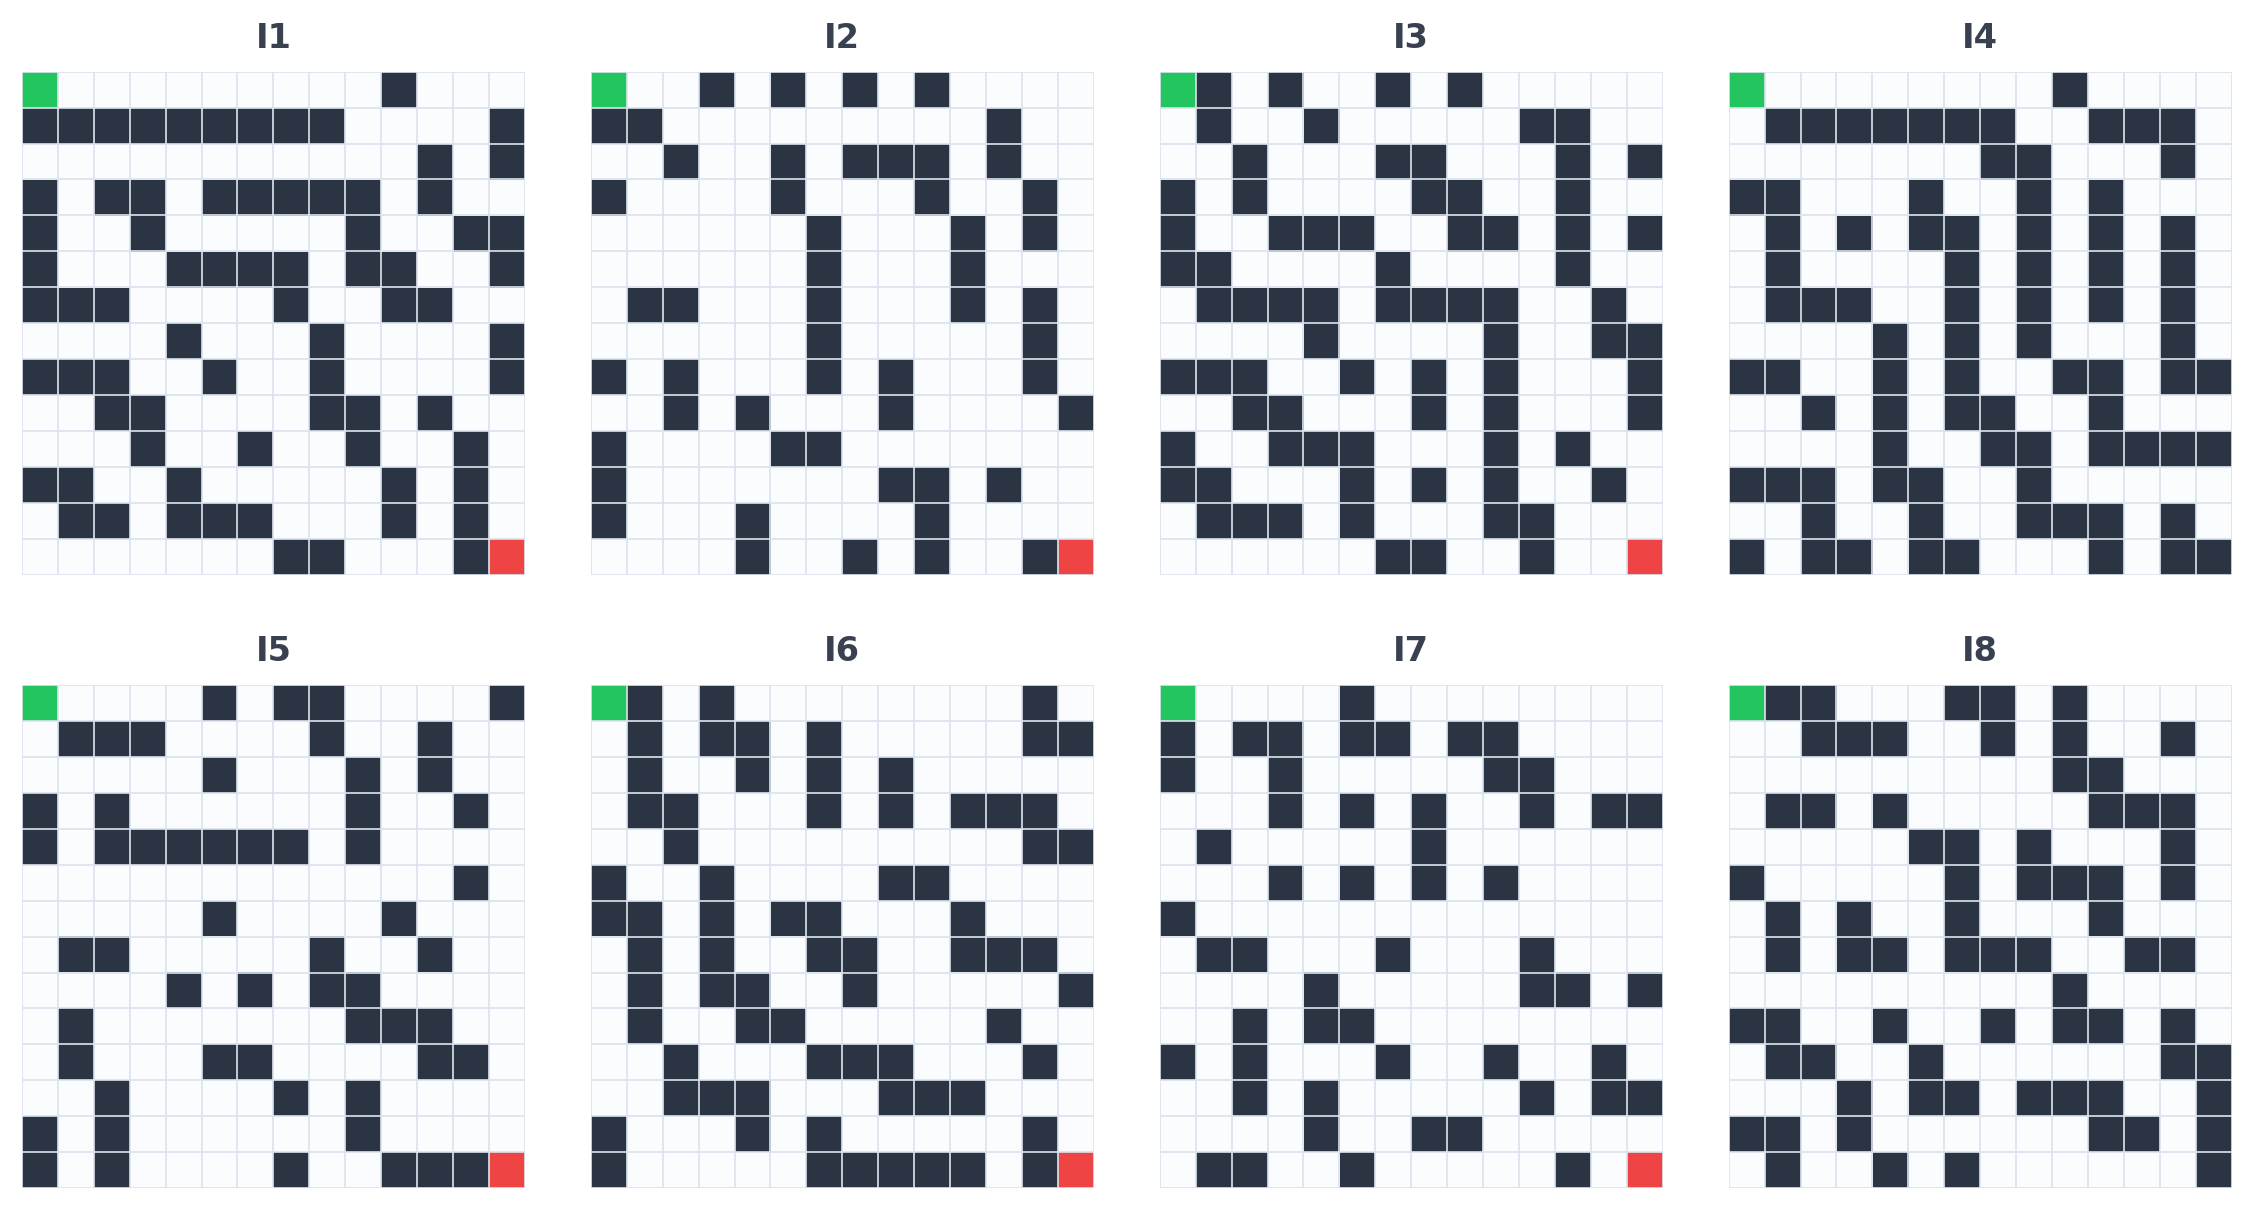
\includegraphics[width=0.92\textwidth]{figures/pcgnn/map_improved_samples.png}
    \caption{Mẫu bản đồ sinh từ genome \emph{winnerseed0.pkl}: đa dạng cấu trúc (hành lang dài, vùng mở, vật cản trung tâm) trước bước phân tầng độ khó.}
    \label{fig:pcgnn_inctyseed0_maps}
\end{figure}

Chỉ số khả năng giải trong thiết lập mê cung không áp dụng trực tiếp ở đây vì tiêu chí đó kiểm tra đường đi giữa hai góc cố định, còn đề tài yêu cầu vùng sàn liên thông đủ rộng để chiến đấu -- hai yêu cầu khác nhau. Vì vậy đề tài thay bằng tỷ lệ sàn liên thông.

\subsection{Nạp bản đồ vào Unity}

TilemapGenerator.cs đọc text asset theo tham số \textbf{difficulty} truyền từ ML-Agents, dựng tilemap, chạy BFS để xác nhận vùng đi được và chọn vị trí sinh. Chế độ vị trí sinh cố định (difficulty 0--2) ưu tiên ô sàn có vùng BFS rộng; chế độ vị trí sinh ngẫu nhiên (difficulty 3) lấy ngẫu nhiên từ sàn hợp lệ với \textbf{randomEnemySpawnCount}=2.

\section{Hiện thực tác nhân CombatAgent}

CombatAgent.cs là lớp trung gian giữa gameplay của TopDown Engine và vòng lặp học của ML-Agents. Về phía Unity, lớp này đọc trạng thái nhân vật, kẻ địch, đạn và bản đồ; về phía trainer, nó cung cấp vector quan sát, nhận hành động do chính sách sinh ra, áp dụng hành động vào nhân vật và trả lại phần thưởng. Cách tách này giúp giữ phần logic học tăng cường nằm trong một thành phần rõ ràng, trong khi các hệ thống có sẵn của game như di chuyển, vũ khí, máu và dash vẫn được tái sử dụng.

\subsection{Vòng đời lượt chơi}

CombatAgent kế thừa lớp \textbf{Agent} của ML-Agents. Ở đầu mỗi lượt chơi, hàm \textbf{OnEpisodeBegin} đặt lại các biến thống kê, cập nhật trạng thái vũ khí, sinh hoặc nạp lại phòng thông qua TilemapGenerator nếu cấu hình yêu cầu, sau đó đưa người chơi và kẻ địch về trạng thái hợp lệ. Lượt chơi kết thúc khi người chơi bị hạ, toàn bộ kẻ địch bị tiêu diệt, hoặc môi trường rơi vào trạng thái lỗi như nhân vật/kẻ địch bị đẩy ra ngoài vùng chơi. Các trường hợp lỗi được xử lý riêng bằng hình phạt nhỏ hoặc kết thúc sớm để tránh đưa quá nhiều mẫu nhiễu vào bộ nhớ huấn luyện.

Trong mỗi bước quyết định, CombatAgent thực hiện ba thao tác chính: thu thập quan sát bằng \textbf{CollectObservations}, giới hạn các hành động không hợp lệ bằng \textbf{WriteDiscreteActionMask}, và xử lý hành động trong \textbf{OnActionReceived}. Ba hàm này tương ứng trực tiếp với ba thành phần của bài toán RL: trạng thái quan sát $s_t$, hành động $a_t$ và phần thưởng $r_t$.

\subsection{Thu thập quan sát}

Trong các cấu hình thí nghiệm cơ sở, \textbf{CollectObservations} tạo vector 207 chiều như Bảng~\ref{tab:obs_207}. Vector này gồm bốn nhóm thông tin: trạng thái người chơi, thông tin tổng quát của cảnh chơi, danh sách kẻ địch/đạn gần nhất và 16 tia dò tường xung quanh tác nhân. Việc dùng vector cấu trúc thay cho ảnh pixel giúp giảm chi phí học, đồng thời làm rõ tác động của curriculum learning và các kỹ thuật hỗ trợ như ICM, RND, LSTM.

Nhóm trạng thái người chơi mã hóa các tín hiệu cần cho chiến đấu ngắn hạn: máu hiện tại, đạn hoặc tài nguyên vũ khí, thời gian hồi chiêu, trạng thái sẵn sàng tấn công, vận tốc và dấu hiệu vừa nhận sát thương. Nhóm thông tin toàn cục ghi lại tỷ lệ kẻ địch/đạn đang nhìn thấy và thời gian đã trôi qua trong lượt chơi, giúp chính sách phân biệt giữa giai đoạn đầu và cuối episode.

Với kẻ địch, CombatAgent lấy tối đa ba kẻ địch gần nhất trong bán kính quan sát, sắp xếp theo khoảng cách rồi mã hóa từng kẻ địch bằng các đặc trưng như vị trí tương đối, vận tốc tương đối, khoảng cách chuẩn hóa, lượng máu và mức đe dọa ước lượng. Nếu số kẻ địch quan sát được ít hơn giới hạn này, các vị trí còn lại được điền bằng 0. Cơ chế đệm này cũng được dùng cho nhóm đạn, trong đó tối đa mười viên đạn gần nhất được mô tả bằng vị trí tương đối, vận tốc, khoảng cách và thời gian ước lượng tới va chạm. Nhờ vậy, kích thước đầu vào của mạng luôn cố định dù số đối tượng trong cảnh thay đổi theo từng lượt chơi.

Riêng với kẻ địch, bán kính quan sát không chỉ là một vùng tròn vật lý quanh tác nhân. Sau khi lấy các đối tượng nằm trong \emph{VisionRadius}, hệ thống còn kiểm tra đường nhìn trực tiếp tới mục tiêu bằng raycast trên lớp tường; vì vậy, kẻ địch bị vật cản che khuất sẽ không được xem là mục tiêu hợp lệ. Với đạn, hệ thống ưu tiên cung cấp tín hiệu né tránh kịp thời nên thu thập các projectile nằm trong bán kính quan sát mà không áp dụng cùng điều kiện đường nhìn như kẻ địch.

Nhóm tường/vật cản dùng 16 tia ray tỏa đều quanh tác nhân để đo khoảng cách tới tường gần nhất. Đây là biểu diễn gọn, nhưng chỉ phản ánh vật cản cục bộ theo từng hướng. Vì vậy, các thí nghiệm mở rộng sau này kiểm tra thêm hai cách bổ sung thông tin không gian: run59 thêm đặc trưng đường đi BFS vào quan sát, còn run62 bổ sung lưới chiếm chỗ cục bộ $15\times15$ để chính sách nhìn được cấu trúc sàn/tường quanh tác nhân.

\subsection{Không gian hành động và action mask}

Đầu ra của chính sách là bốn nhánh hành động rời rạc $(3,3,3,9)$: di chuyển theo trục X, di chuyển theo trục Y, lựa chọn chiến đấu và hướng ngắm. Hai nhánh di chuyển tạo thành chín khả năng di chuyển cơ bản, gồm đứng yên và tám hướng trên mặt phẳng. Nhánh chiến đấu gồm không hành động, tấn công và dash. Nhánh ngắm gồm giữ hướng hiện tại hoặc chọn một trong tám hướng rời rạc.

Hàm \textbf{WriteDiscreteActionMask} được dùng để loại bỏ một số hành động rõ ràng không hợp lệ trước khi chính sách lấy mẫu. Ví dụ, hành động tấn công bị che khi vũ khí chưa sẵn sàng hoặc không có mục tiêu phù hợp; hành động dash có thể bị che khi xung quanh không có mối đe dọa cần né. Action mask không thay tác nhân quyết định chiến thuật, nhưng giúp giảm số mẫu lãng phí do các hành động không thể thực thi, đặc biệt trong giai đoạn đầu khi chính sách còn gần ngẫu nhiên.

Trong \textbf{OnActionReceived}, bốn nhánh hành động được giải mã thành vector di chuyển, hướng ngắm và lệnh chiến đấu. CombatAgent sau đó gọi các thành phần của TopDown Engine để áp dụng di chuyển, xoay hướng nhân vật, kích hoạt vũ khí hoặc dash. Một số cấu hình huấn luyện có thêm cơ chế hỗ trợ căn hướng khi tấn công mục tiêu hiện tại; cơ chế này nhằm giảm nhiễu do thao tác ngắm quá thô trong giai đoạn học ban đầu, trong khi chính sách vẫn phải tự học thời điểm tiếp cận, tấn công, né tránh và giữ khoảng cách.

\subsection{Tính thưởng và ghi log hành vi}

Phần thưởng được tính trực tiếp trong \textbf{OnActionReceived} dựa trên thay đổi trạng thái giữa hai bước quyết định liên tiếp. Với mục tiêu chiến đấu, hệ thống theo dõi tổng máu của kẻ địch và số kẻ địch còn sống. Khi tổng máu giảm, tác nhân nhận thưởng gây sát thương; khi số kẻ địch giảm, tác nhân nhận thưởng tiêu diệt; khi không còn kẻ địch sống trong phòng, tác nhân nhận thêm thưởng dọn phòng và episode kết thúc. Cách tính này bám sát mục tiêu thật của trò chơi: gây sát thương chỉ là tín hiệu trung gian, còn hạ kẻ địch và dọn phòng mới là kết quả cần tối ưu.

Bên cạnh phần thưởng kết quả, CombatAgent còn dùng một số tín hiệu định hình nhỏ để giúp PPO học ổn định hơn. Tác nhân được thưởng khi tiến gần mục tiêu, căn hướng tấn công tốt hoặc dùng dash trong tình huống có nguy cơ; ngược lại, nó bị phạt khi nhận sát thương, đứng gần kẻ địch nhưng không hành động, tấn công sai thời điểm hoặc lặp lại các hành động không hợp lệ. Ở các cấu hình có \texttt{aggressive\_seek}, tác nhân còn nhận tín hiệu khuyến khích tiếp cận kẻ địch theo khoảng cách đường đi, giúp giảm các tình huống đứng yên hoặc đi vòng quanh khi chưa có đường ngắm trực tiếp.

Ngoài tổng phần thưởng, CombatAgent ghi thêm các chỉ số hành vi vào TensorBoard như \textit{kills/episode}, \textit{clear\_rate}, \textit{damage\_dealt}, \textit{damage\_taken}, tỷ lệ tấn công đúng hướng, tỷ lệ tấn công không hợp lệ và tỷ lệ dash hữu ích. Các chỉ số này rất cần thiết khi phân tích kết quả: một cấu hình có reward cao hơn chưa chắc đã chiến đấu tốt hơn nếu reward tăng do tín hiệu định hình; ngược lại, các chỉ số như số kẻ địch tiêu diệt, tỷ lệ dọn phòng và sát thương gây ra cho biết chính sách có thật sự học được hành vi chiến đấu hay không.

\section{Cấu hình huấn luyện PPO}

Cấu hình PPO được chuẩn hóa để làm nền so sánh cho các lần chạy ablation, đặc biệt là nhóm dùng curriculum learning từ run46 trở đi. So với các thử nghiệm ngắn ban đầu, các lần chạy chính tăng lên 1--3 triệu bước vì môi trường sinh theo thủ tục tạo phân phối trạng thái rộng hơn nhiều so với một bản đồ cố định. Nếu số bước quá thấp, tác nhân có thể chỉ học được các phản xạ cục bộ như tiến gần hoặc bắn khi thấy mục tiêu, nhưng chưa đủ dữ liệu để ổn định chuỗi hành vi dài gồm tiếp cận, né đạn, căn hướng và kết liễu kẻ địch.

Các tham số PPO được chọn theo hướng ưu tiên ổn định hơn là tốc độ hội tụ tức thời. \emph{buffer\_size} và \emph{batch\_size} đủ lớn để mỗi lần cập nhật chứa nhiều tình huống khác nhau; \emph{time\_horizon}=64 giữ lại chuỗi trải nghiệm đủ dài cho các phần thưởng trễ như hạ kẻ địch hoặc dọn phòng; hệ số entropy $\beta$ được giữ ở mức vừa phải để chính sách còn khám phá trong không gian hành động nhiều nhánh nhưng không duy trì ngẫu nhiên quá lâu.

\begin{table}[H]
    \centering
    \small
    \caption{Cấu hình PPO dùng trong các lần chạy chính}
    \label{tab:ppo_baseline_config}
    \begin{tabular}{|p{4cm}|c|p{7cm}|}
        \hline
        \textbf{Tham số} & \textbf{Giá trị} & \textbf{Ghi chú} \\
        \hline
        trainer\_type & ppo & Thuật toán chính. \\
        \hline
        batch\_size & 1024 & Kích thước minibatch khi cập nhật chính sách. \\
        \hline
        buffer\_size & 10240 & Số bước trải nghiệm thu thập trước mỗi lần cập nhật PPO. \\
        \hline
        learning\_rate & $3.0 \times 10^{-4}$ & Linear schedule. \\
        \hline
        beta & $5.0 \times 10^{-3}$ & Hệ số entropy bonus. \\
        \hline
        epsilon & 0.2 & Ngưỡng clipping của PPO. \\
        \hline
        lambd & 0.95 & GAE. \\
        \hline
        num\_epoch & 3 & Số epoch trên mỗi buffer. \\
        \hline
        hidden\_units & 256 & Mạng MLP actor-critic. \\
        \hline
        num\_layers & 2 & Hai lớp ẩn. \\
        \hline
        time\_horizon & 64 & Độ dài trajectory trước khi cập nhật. \\
        \hline
        max\_steps & 1M hoặc 3M & 1M cho cấu hình cơ sở, 3M cho curriculum chính. \\
        \hline
    \end{tabular}
\end{table}

Các cấu hình phần thưởng nội tại bổ sung tín hiệu nội tại từ ICM hoặc RND. Các cấu hình LSTM thêm bộ nhớ có kích thước 256 và chuỗi quan sát dài 64 bước. Các cấu hình curriculum thêm tham số \texttt{environment\_parameters.difficulty} để trainer tự chuyển bài học dựa trên phần thưởng đã làm mượt. Nhờ giữ nguyên phần lớn tham số PPO giữa các lần chạy, các khác biệt ở Chương~4 có thể được quy về yếu tố đang kiểm tra thay vì bị lẫn với thay đổi cấu hình huấn luyện.

\section{Thiết kế thí nghiệm loại trừ}

Mỗi nhóm thí nghiệm loại trừ chỉ thay đổi một yếu tố chính so với cấu hình tham chiếu. Mục tiêu không phải tìm tổ hợp tối ưu tuyệt đối, mà là xác định yếu tố nào thực sự tạo cải thiện trên môi trường chiến đấu sinh theo thủ tục.

\begin{table}[H]
    \centering
    \small
    \caption{Ma trận thí nghiệm loại trừ chính}
    \label{tab:ablation_matrix_design}
    \begin{tabular}{|p{2cm}|p{5.1cm}|c|p{5.2cm}|}
        \hline
        \textbf{Run} & \textbf{Thiết lập} & \textbf{Mốc huấn luyện} & \textbf{Mục đích} \\
        \hline
        run34 & PPO cơ sở & 1.0M & Mốc so sánh không curriculum, không phần thưởng nội tại. \\
        \hline
        run35 & PPO + ICM & 1.0M & Kiểm tra động lực nội tại (intrinsic motivation) theo Pathak et al. \cite{Pathak2017}. \\
        \hline
        run36 & PPO + RND & 1.0M & Kiểm tra động lực nội tại (intrinsic motivation) theo Burda et al. \cite{Burda2018}. \\
        \hline
        run42 & PPO + LSTM & 1.0M & Kiểm tra lợi ích của kiến trúc bộ nhớ \cite{Hochreiter1997}. \\
        \hline
        run46 & PPO + Curriculum & 3.0M & Đánh giá tác động của curriculum learning. \\
        \hline
        run47 & Curriculum + LSTM & 3.0M & Đánh giá LSTM khi kết hợp với curriculum. \\
        \hline
        run50 & Curriculum + ICM & 3.0M & Đánh giá ICM khi kết hợp với curriculum. \\
        \hline
        run54 & 4 bậc, cố định--ngẫu nhiên & 3.0M & Kiểm tra giảm phương sai vị trí sinh đầu huấn luyện. \\
        \hline
        run55 & Curriculum + hàm thưởng v2 & 3.0M & Kiểm tra thay đổi thang thưởng và tăng trọng số kết quả. \\
        \hline
    \end{tabular}
\end{table}
Mỗi lần chạy trong ma trận trên được chạy một seed và dừng khi chính sách đã hội tụ. Vì giới hạn này, các kết quả ở Chương~4 được diễn giải như xu hướng thực nghiệm, tránh khẳng định quá mức với các chênh lệch nhỏ.

Ngoài ma trận ablation chính, đề tài thực hiện thêm hai lần chạy mở rộng 
về biểu diễn quan sát.

\textbf{Run59 (path-informed).} Sau khi các lần chạy 207 chiều dừng ở vùng bão hòa entropy khoảng 4.40 nat, đề tài đặt giả thuyết giới hạn nằm ở biểu diễn quan sát, không phải thuật toán. Run59 kiểm tra giả thuyết này bằng cách bổ sung ba tín hiệu BFS vào vector quan sát (lên 210 chiều): hướng bước kế tiếp và khoảng cách chuẩn hóa tới kẻ địch gần nhất. Khác với 16 tia ray chỉ phản ánh tường tức thời, tín hiệu BFS mang thông tin đường đi toàn cục. Vì vậy run59 không được xem là cấu hình end-to-end thuần túy, mà là một ablation có chủ đích để đo xem thông tin điều hướng ảnh hưởng mạnh đến hiệu năng đến mức nào.

\textbf{Run62 (lưới cục bộ, 40.82M bước).} Run62 đi theo hướng thận trọng hơn run59: thay vì đưa trực tiếp hướng đi BFS vào quan sát, cấu hình này bổ sung lưới chiếm chỗ cục bộ $15\times15$ (225 chiều) để tác nhân tự khai thác cấu trúc sàn/tường quanh mình. Tổng kích thước quan sát tăng lên \textbf{432 chiều}. Cấu hình này đồng thời dùng curriculum 4 bậc, ICM (strength 0.001), bật tham số \texttt{aggressive\_seek}, chạy 8 môi trường song song và được huấn luyện 40.82M bước trong hai phiên liên tiếp. Vì run62 thay đổi nhiều yếu tố cùng lúc, kết quả của nó được xem là thí nghiệm thăm dò mở rộng: cho thấy hướng biểu diễn không gian có tiềm năng, nhưng chưa đủ để kết luận riêng lưới cục bộ là nguyên nhân duy nhất tạo cải thiện.

\begin{table}[H]
    \centering
    \small
    \caption{Các tham số PPO khác biệt của run62 so với cấu hình cơ sở}
    \label{tab:run62_ppo_config}
    \begin{tabular}{|p{4cm}|c|c|p{5cm}|}
        \hline
        \textbf{Tham số} & \textbf{Cấu hình cơ sở} & \textbf{run62} & \textbf{Ghi chú} \\
        \hline
        VectorObservationSize & 207 & 432 & Thêm lưới cục bộ (local occupancy grid) 15$\times$15 (225 chiều). \\
        \hline
        batch\_size & 1024 & 2048 & Tăng để ổn định gradient với quan sát lớn hơn. \\
        \hline
        buffer\_size & 10240 & 20480 & Tăng tương ứng với batch\_size. \\
        \hline
        learning\_rate & $3.0 \times 10^{-4}$ & $5.0 \times 10^{-5}$ & Giảm để tránh bước cập nhật quá lớn. \\
        \hline
        num\_epoch & 3 & 2 & Giảm để tránh quá khớp trên buffer. \\
        \hline
        max\_steps & 1M -- 3M & 50M (mục tiêu) & Chạy thực tế đến 40.82M bước. \\
        \hline
    \end{tabular}
\end{table}
